\chapter[Neutral MSSM Higgs Search...]{The Search for neutral MSSM Higgs Bosons in the final state:
$\tau^{+}\tau^{-} \rightarrow e \mu + 4\nu$}

Discovering the mechanism responsible for electroweak
symmetry-breaking and the origin of mass for elementary particles has been
one of the major goals of the physics program at the Large Hadron
Collider~(LHC)~\cite{LHC}.  In the Standard Model (SM) this mechanism
requires the existence of a single scalar particle, the Higgs
boson~\cite{ENGLERT,HIGGS,HIGGS2,HIGGS3,Guralnik:1964eu}.
%The recent discovery of a particle with mass close to 125~GeV at the LHC with properties that resemble
%the ones of the Higgs boson~\cite{ATLASHiggsObservationJuly2012,CMSHiggsObservationJuly2012}
%is also compatible with several extension of the SM, and in particular with Super Symmetry (SUSY) scenarios~\cite{theo125,theo125_v2}. 
%When calculating radiative correction to the Higgs
%mass one encounters divergences, for the Higgs mass to be finite
%counter-term has to be added and a fine-tuning between the counter term and the divergences has to take place, this 
%is what is called the naturalness \cite{} problem. 
%Introduction of Super Symmetry (SUSY), a new symmetry that connects bosons and fermions, solve this problem. 
%the MSSM under the assumption that is a SM-like Higgs boson that can be 
%identified with one of  MSSM neutral Higgs bosons~
In the Minimal Supersymmetric extension of the Standard Model
(MSSM)~\cite{MSSM1, MSSM2} the Higgs sector is composed of two Higgs
doublets of opposite hyper-charge, resulting in five observable Higgs
bosons.  Two of these Higgs bosons are neutral and $CP$-even
($h$,$H$), one is neutral and $CP$-odd ($A$) and two are charged
($H^\pm$).  At tree level their properties such as masses, widths and
branching ratios can be predicted in terms of only two parameters,
often chosen to be the mass of the $CP$-odd Higgs boson $m_A$, and
the ratio of the vacuum expectation values of the two Higgs doublets
$\tan\beta$.  For relatively large values of $\tan\beta$ one of the
$CP$-even Higgs bosons is almost degenerate in mass with
$A$. Moreover, Higgs couplings to down (up) type fermions are enhanced
(suppressed) by $\tan\beta$, meaning that for large $\tan\beta$
bottom-quark and $\tau$ lepton will play a more important role than in
the SM case either for production and decay.

%\clearpage
The production of the neutral $CP$-even MSSM Higgs bosons at hadron
colliders proceeds via the same processes as for the SM Higgs
production. However, the pseudoscalar $A$ instead cannot be produced
in association with gauge bosons or in vector boson fusion (VBF) at
tree-level, as this coupling is forbidden due to $CP$-invariance.  At
the LHC one of the most relevant production mechanisms for the MSSM
Higgs bosons is gluon-gluon fusion, $gg\rightarrow A/H/h$. In
addition, the production in association with $b$-quarks becomes
important for large value of $\tan\beta$ .  The decays of the neutral
MSSM Higgs bosons (in the assumption that all supersymmetric particle
are heavy enough) are the same as for the SM one with the already
cited exception of $A$, however the decay rates depend on a large
extent to the couplings with fermions and gauge bosons.

Searches for neutral MSSM Higgs bosons have been performed at
LEP~\cite{LEPLimits}, the
Tevatron~\cite{TevatronLimits1,TevatronLimits2,TevatronLimits3,TevatronLimits4,TevatronLimits5,TevatronLimits6}
and the LHC~\cite{CMSLimit, ATLASLimit}.  In this note a search for
neutral MSSM Higgs bosons with the ATLAS experiment at CERN is
presented, using proton-proton collisions at centre-of-mass energy of
8~TeV, with a recorded integrated luminosity of
$20.3 \ifb$.
The results of this search are interpreted in a model independent
fashion, as limits on the product of the cross section and branching
ratio for such a new particle, as well a limits on the MSSM in the
$m_{h}^{max}$ scenario \cite{MSSMmhmax}. Only b-quark associated and
gluon fusion are considered as production mode for the Higgs bosons, the search then focuses
on the subsequent decay into a
$\tau^+\tau^-$ pair. Furthermore, only cases in which both $\tau$
decays leptonically, with one decaying to an electron and the other to
a muon, are considered. This final state corresponds to a total
$\tau^+\tau^-$ branching ratio of approximately 6\%.
%However, due to the reduced QCD background, 
%this search can still compete with the hadron-hadron and the
%lepton-hadron cases. 
The analysis strategy is to
split the selected events in two categories by requesting the presence
(b-tag) or absence (b-veto) of a jet coming from a $b$-quark. This
solution helps to separate the contribution of the two production modes
and allows for optimisation of selections due to the 
different backgrounds for the different final states..

The signal topology is characterised by a final state with an
electron, a muon, and missing transverse energy due to the
presence of four neutrinos from the $\tau$ decays. Furthermore, the
final state may be split by the presence or
absence of a $b$-quark initiated jet, depending on the production
process.  The background processes which are considered in this study
are the production of $W$ and $Z$ bosons in association with
jets~($W/Z$+jets), pairs of top quarks~(\ttbar), single top
quark~(the so-called single-top) and pairs of electroweak gauge
bosons~($WW, WZ, ZZ$). Finally QCD multi-jet also forms a non-negligible
background due to its large production cross-section. Where possible
these backgrounds are estimated using data driven methods.

This note is structured as follows: The ATLAS detector is briefly
described in Section~\ref{sec:ATLAS}. In Section~\ref{sec:data_mc} the
collision data set, the Monte Carlo-simulated event samples as well as
hybrid (tau-embedded) data samples used in this study are
described. The reconstruction of physics objects, the trigger
requirements and the offline event selection are discussed in
Sections~\ref{sec:presel} and~\ref{sec:eventsel}. Background estimation methods are
described in Section~\ref{sec:BackgroundEstimation}, and the
systematic uncertainties are discussed in
Section~\ref{sec:Systematics}. A statistical analysis and resulting
exclusion limits are described in Section~\ref{sec:Results}, followed
by conclusions in Section~\ref{sec:Conclusions}.
Search of MMSM Higgs bla....
This chapter is divided in three sections, in the first one the motivation and the 
analysis strategy is presented, in section~\ref{} are discussed the problematics 
that arise when real data enters the game and ideas to estimate backround are needed, 
as well as systematics, in section~\ref{}  focus is set on results with a small introduction to
statistical methods.


In this section we make use of analysis tools described in chapter~\ref{c:detector}, as well
we refer to objetc definition made in this chapter (like electron reconstruction, jet difinition, muons, ecc.).

%\section{Inside Neutral MSSM Higgs}
%\section{What is a Search?}
%\section{Search First Principle}
%\section{Search Elements}
%\section{The Search in a Nutshel}
\section{The Search Strategy}

\subsection{Motivation}
Under the light of the recent discovery of a Higgs boson with mass of 125 GeV, is very reasonable
to ask ourselfs if all the piece of the Higgs sector have been discovered, if there is nothing missing
to complete the puzzle. Indeed such a new particle can be accomodated within several beyond the 
standard model scenario, this is particularly true in the MSSM. 
Talk about mhmod....
Figure~\ref{} shows 

\subsection{How to search for new phenomena?} 
%\subsection{What is a search?} 
Statistical statement associated to the claim of discovery for new physics \cite{Cramer_LHC}. Typically new physics searches are looking for a signal 
that is additive on top of the background. Discovery is formulated in terms of an hypotesis test where the background-only hypotesis
plays the role of the null hypotesys and the signal+background hypotesis plays the role of the alternative. A very simple example:
a \emph{signal region} is defined where events are counted, the events are distributed with a poisson distribution 
of which the mean value (the number of expected events) is defined for each of the two hypotesis, one expects $\nu_{B}$ events 
$H_{0}$ and $\nu_{B} + \nu_{S}$ for the $H_{1}$ alternative hyspotesis. The number of observed events n is a random
variable described by a Poisson distribution, then the probability model for null and the alternate hypotesis is respectively 
$\text{Pois}(n|\nu_{B})$ and $\text{Pois}(n|\nu_{B} + \nu_{S})$.
Let assume to observe in data $N_{SR}$ events, it is obvious that evidence for a signal shows up as an excess of 
events, a way to quantify the conpatibility of the null hypo with data
is to make a \emph{significance} test, this leads to the calculation of the probability that the background-only would produce at least as many
as the observed events, this is the definition of p-value, which in this case would be expressed by the formula:
$$
\text{p-value} = \sum_{n=N_{SR}}^{\infty} \text{Pois}(n|\nu_{B})
$$
Calculating  p-value is a way to characterize an excess, prob that..., but what about the case there is no excess?
We want to estimate the exclusion limit for teh signal hypo, we want to accept the null hypo and at the same time reject 
the signal hypo with a fixed predetermined probability (called confidence level). Neuman-Person define a framework with a
set of rules to achieve this.

It often used a so-called discriminating variable to help separating signal and backgrounds, this can be any of the observables of
the experiment, usually chosen invariant mass of final state particle, or MVA or ecc., let's call this observable X, one can complete
the above mentioned statistical model for the two hypotesis by using the probability distribution of X for background and signal process
$$
\text{Pois}(N_{SR}|\nu) \prod_{i}^{N_{SR}} f(e_{i} | \vec{\theta})
$$
With this one can use the full power of the prediction of the probability model to disentangle between signal and background.
A statistical test is a rule that define a region in parameter space for which  a given hypotesis can be accepted or rejected.
Often rather than using a full set of data $\vec{X}$, it is convenient to define a \emph{test statistic}, t, which is usually a single
number, it is a quantity calculated out of the data, a mapping of a set of measurements into a single number. The test statistic, that is usually
connected to the discriminating variable, would then have a different distribution for the different hypotesis, one can then define $\alpha$
called the size of the test and $t_{\alpha}$ for which $P(t < t_{\alpha} | H_{0}) \leq \alpha$ then in this case $H_{0}$ is rejected.

- Alternative: NP provided a framework for hypotesis testing that addresses the choice of the test statistic. First one defines 
an acceptance region in terms of a test statistic, such that if $T(\vec{X}) < t_{\alpha}$ one accepts the null hypotesis. 
One can think of $T(\vec{X}) = t_{\alpha}$ as a counturn in the space of the data which is the boundary to this acceptance region.
Then one defines the size of the test $\alpha$ which is the probability for the null hypotesis to be rejected when true,
the test is totally asymmetric: if the null hypotesis is rejected then the alternate is accepted (is this true??)....

Summarizing there are different building blocks for a search:
\begin{itemize}
	\item Define a signal region in data where signal is enhanced with respect to the backgrounds, detailed in section \ref{bla}
	\item Define a discriminating variable which is usefull to disentangle between signal and backgrounds, section \ref{bla}
	\item Define the probability model, i.e., the expectation for background and signal, this is one of the most importat
		point of a search and main part of the work of this thesis, detailed in section \ref{bla}
	\item Define a test statistics, which is detailed for the LHC in section \ref{bla}.
\end{itemize}


-----------------------------------------------------------


The language of searching for new phenomena is statistics, the aim of a search is to exclude certain region of parameter space for a 
defined model or (this is quantified by) observe an excess... Statistical methods define procedure for characterising  
an observation of excess or exclusion of a signal.
Frequentist hypotesis test provide a rule for accepting or rejecting hypotesis depending on the outcome of a measurement.

To compare the compatibility of the data with the background-only and signal+background hypoteses a so called test statistic is constructed.

An Hypotesis is a statement about the distribution of the data, a \emph{statistical test} is a rule used to reject or accept an hypotesis.
This is done defining a parameter space, a region 

We use the Neyman-person hypotesis test to set exclusion limits, to characterize instead the significance of an observation we use the p-value.
With some test statistics one can set a region with fixed probability for the signal to occurr, one can then accept-reject this hypotesis with
fixed probability, the test is symmetric: rejecting $H_{0}$ means accept $H_{1}$.

Si ma si parla sempre di numero di eventi.... Fare esempio concreto!

Frequentist hypo test ---> 2 hypo necessary
*) search e' una cifra di cose, nella stostra accezione una search significa looking for excess of events with a particular topology.
The language of a search is statistics so we are going to define some quantities:
*) Test of hypotesys: define a test to say if this hypo is true
*) calculate the probability, under the hypo, to observe a deviation at least as big as the one observed in data, this is the definition of p-value.
This is usefull in case you do have a signal, what about if not?
*) you define an additional hypotesis, signal hypo, and ten you can exclude a certain range of parameter space with a pre-fixed probability.
*) Il tutto si riduce a contare eventi nella signal region. Next sections define how we built this signal region and why.

Some statistical definitions Hypotesys 0, bla bla...
Bump search

generalita' of a statistical model





\subsection{Signal Topology}
Way to inhance signal that gives you sensitivity increase (b-tag, b-veto)
Higgs BR and production

\subsection{How to deal with Backgrounds}
%\subsection{Selections}
%This may go in previos subsection %%%%%%%%%%%%%%%%%%%%%%%%%%%%%%%%%%%%%%%%%%%%%%%%%%%%%%%%%%%%%%%%%%%%%%%%%%%%%%%%%%%%%%%%%%%%%%
%The signal topology described above translates in terms of an "experimental" point of view in requiring			%
%Trigger, exactly one electron, exactly one muon, of opposite charge and isolated. With isolation				%
%it's meant that in a cone around the lepton there should be little energy deposit (should not be sorraunded by 		%
%other particle - common of non-promt leptons coming from jets). More detail about isolation properties and			%
%variable are detailed in section ~\ref{sec:bkg}. Full detail on actual preselections regarding all the quality requirements	%
%on object reconstruction are reported in appendix~\ref{ap:presel}.								%
%%%%%%%%%%%%%%%%%%%%%%%%%%%%%%%%%%%%%%%%%%%%%%%%%%%%%%%%%%%%%%%%%%%%%%%%%%%%%%%%%%%%%%%%%%%%%%%%%%%%%%%%%%%%%%%%%%%%%%%%%%%%%%%%%

The signal topology described in the previous section common to many other processes, unfortunately 
those have higher cross section than the signal we are looking for,
%magari qui si puo' dire che ci sono diversi metodi per aumentare S/B 
a set of additional selection has been studied to enhance the sensitivity of the search, or in other words,
to increase the signal  to background  ratio. The most important backgrounds to this search are the production of
 $\Ztautau $ + jets, the top quark ($t\bar{t}$ and single top production is intended), diboson production 
(like $WW$ or $ZZ$ events) and events with non-prompt leptons coming from QCD multi-jet (in short QCD multi-jet).
Vector bosons production like  $\Wlnu$ or $\Zll$ + jets (with l here meanung either $e$ or $\mu$) are also considered,
however those processes have a limited impact.

The final state of Higgs decaying into tau pair coincide with the one from  $\Ztautau$  process, this is then an irreducible 
background, however exploiting the different kinematics of the Higgs decay and the other backgrounds it possible to distinguish 
between signal and them.
%do present different kinematics  and is possible to exploit 
%Exploiting the kinematics of the Higgs deacaying
The most stiking is that the higgs (like $\Ztautau$) selecting an electron and one muon
coming from the tau decay, due to the high mass the taus will be back to back and their decay products will be highly boosted,
this gives rise to two feature: the mu-e will be more likely back to back, as you can see in figure~\ref{fig:selections} that shows the angle between the
leptons in the transverse plane 
$\Delta\phi = |\phi_{e} - \phi_{\mu}| $\footnote{This is actually more complicated: one has to take care of the sign of $\phi$ see chapter\ref{c:detector}}
prefer configuration in wich the leptons are in opposite emisphere.
Furthermore the neutrinos will be more likely collinear with the leptons (given the high boost the taus recive from Higgs decay).
This feature can be matematically seen as the sum of scalar product between missing energy and the leptons four-vectors in the
transverse plane, if the vectors are normalised to unit versors then what remains is a relation only between angles:
$$ \hat{E}_{T}^{miss} \cdot ( \hat{P}_{T}^{\mu} + \hat{P}_{T}^{e} ) = cos(\Delta\phi_{E_{T},\mu}) + cos(\Delta\phi_{E_{T},e})  $$
In the assuption of collinearity and of leptons back-to-back that scalar product  is equal to zero, in fact  it would be equal 
to zero for each of the  neutrinos being it collinear with one lepton and back-to-back with the other.
As can be seen from figure~\ref{fig:selections} in fact the distribution of that variable 
has its more likely values at zero. These two feature can be used to distinguish between mu-e coming from decay from highly 
boosted object and the one coming from W decays in top or in dibosons backgrounds which will have a more spread distribution.
In b-veto category these two selections are sufficient to suppress contribution from dibosons,
no other selection is applied in this category because it has been shown to not bring significant improvement.

In the b-tag category the situation is different, 
the  request of b-jet enhance backgrounds with high jet activity as top production, given the relatively low
jet activity of our Higgs events (also in the case of b-associated production) it's possible to separate them from
top production which instead is very likely to have 2 or more highly enegetic jets in the event, requesting a small jet activity, 
this is achieved by requesting the sum of the jets transverse momentum to be small, we call this variable $\Ht$.
Another feature that distinguish top pair production from Higgs is the much higher invariant mass of the former final state,
in the transverse plane all the leptons will tend to have a higher momentum, we then use the sum of lepton \pt and \met as
a discriminating variable, requesting it to be small. Figure~\ref{} shows the distribution of these two variables 
after the request of a b-jet.

Plots with MMC mass as a function of selection that shows how effective they are in reducing backgrounds.

In table~\ref{} a summary of all the selection variable used with their optimized cut values is reported.
While in table~\ref{} the number of events that survises at each cut stage for different background is reported.

\begin{figure}[htp]
     \begin{center}

            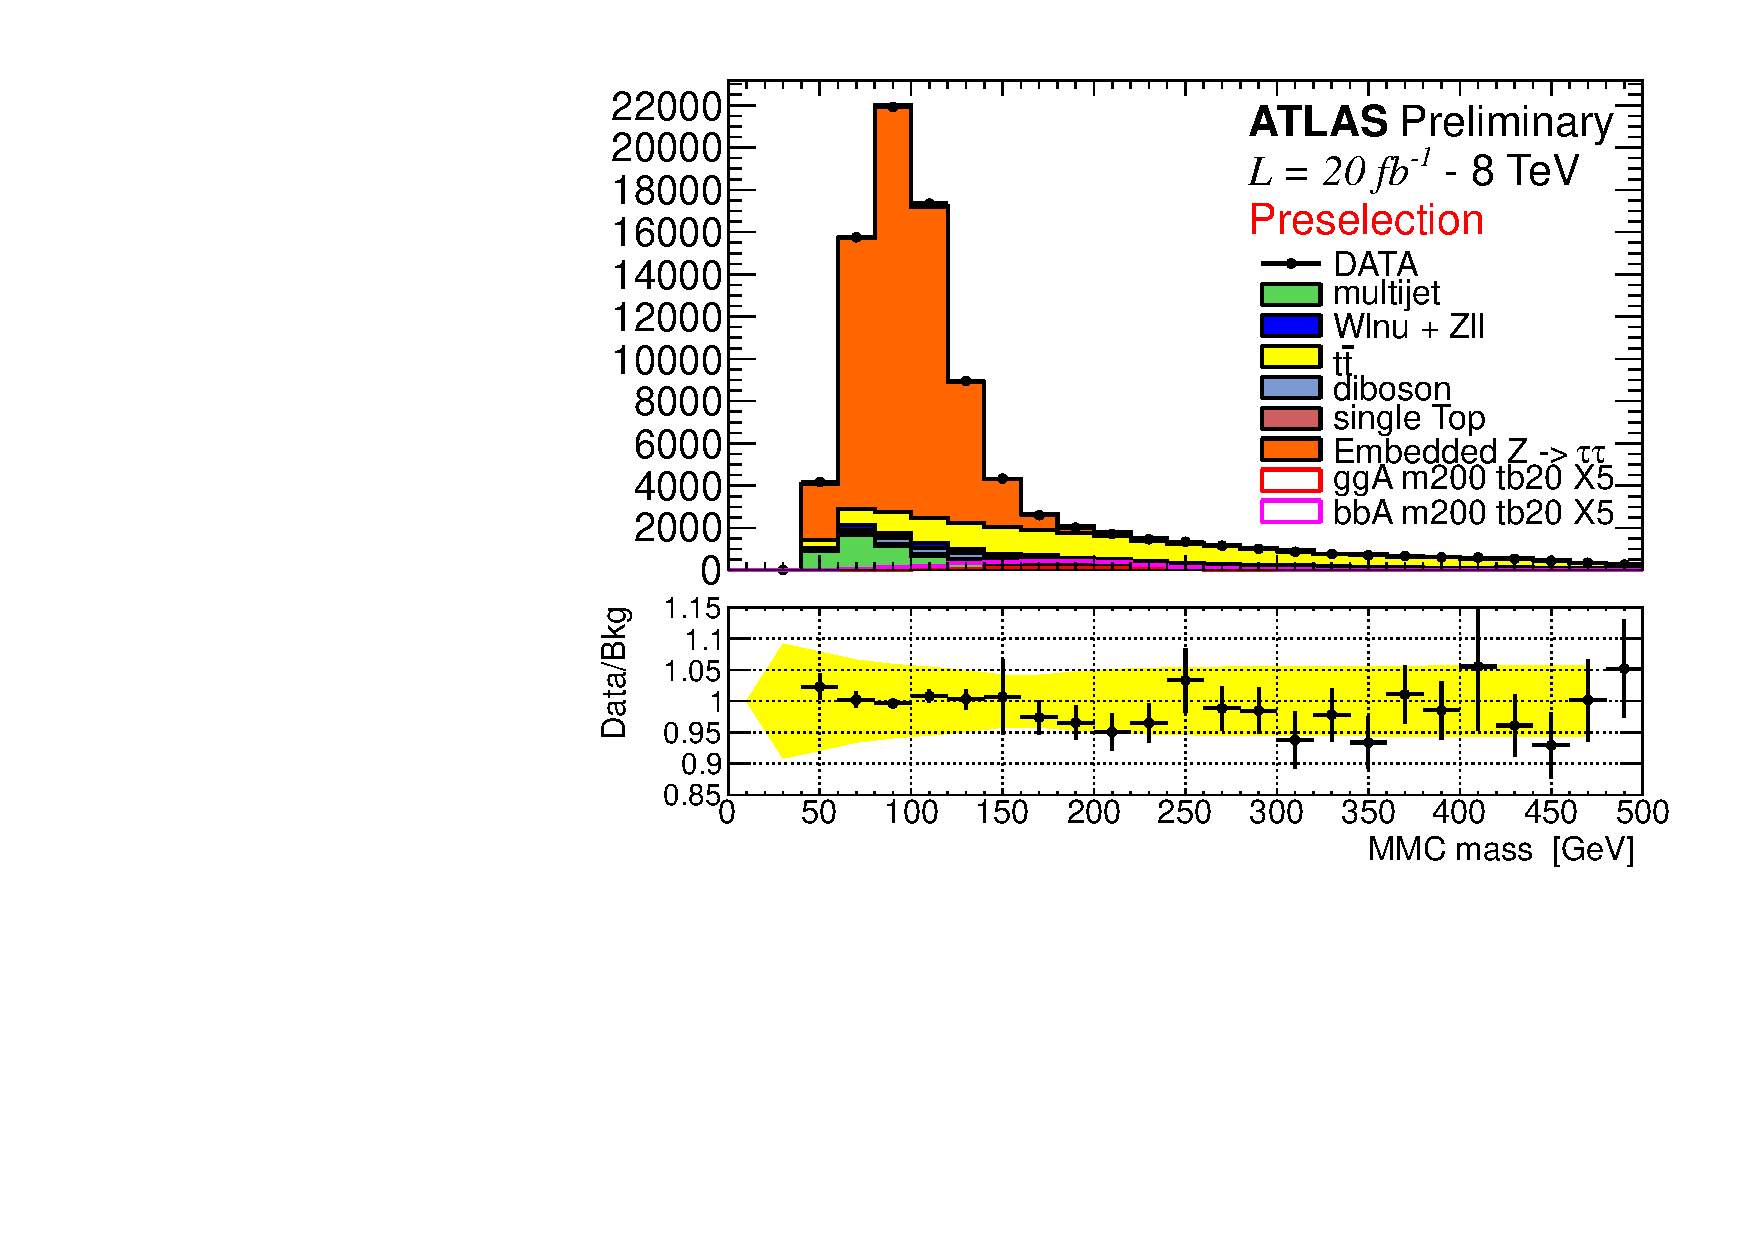
\includegraphics[page=1,width=0.45\textwidth]{figure/std_plots_presel.pdf}
            \includegraphics[page=2,width=0.45\textwidth]{figure/std_plots_presel.pdf}
            \includegraphics[page=3,width=0.45\textwidth]{figure/std_plots_presel.pdf}
            \includegraphics[page=4,width=0.45\textwidth]{figure/std_plots_presel.pdf}
            \includegraphics[page=5,width=0.45\textwidth]{figure/std_plots_presel.pdf}

    \end{center}
    \caption{bla}
   \label{fig:selections}
\end{figure}


\subsection{Missing Mass Calculator}

% si potrebbe anche aggiungere un pezzo di statistica parlando di pdf fatta da histo....
 
Accurate invariant mass reconstruction of a di-tau system is a challenging task due to the escaping neutrinos.
In this analysis, with four neutrinos in the final state, the number of unknown largely exceed the number of constraints,
several approximation are possible to further constraint the neutrinos, for example assuming them collinear to the 
other leptons from tau decay, however those approximation suffers of limitations. 

In this analysis we use the so called missing mass calculator (MMC)~\cite{MMC}
technique for the calculation of the di-tau system invariant mass. This technique employs additional 
information from the well known tau decay to constraint the system, this is achieved by minimising a likelihood function 
defined in the kinematically allowed phase space region, the result is a more precise measurement of the di-tau 
system invariant mass and a considerable improvement in resolution. The invariant mass distribution 
calculated with the MMC technique is referred in the following as $\mmc$ and is used as discriminating 
variable in the limits setting.



